\documentclass{article}
\usepackage{amsmath} %This allows me to use the align functionality.
                     %If you find yourself trying to replicate
                     %something you found online, ensure you're
                     %loading the necessary packages!
\usepackage{amsfonts}%Math font
\usepackage{graphicx}%For including graphics
\usepackage{hyperref}%For Hyperlinks
\usepackage{listings}
\usepackage{graphicx}
\usepackage{natbib}        %For the bibliography
\usepackage{tikz}
\usetikzlibrary{automata, positioning, arrows}
\bibliographystyle{apalike}%For the bibliography
\usepackage[margin=1.0in]{geometry}
\usepackage{float}
\DeclareMathOperator{\EX}{\mathbb{E}}
\graphicspath{ {pictures/} }
\begin{document}
%set the size of the graphs to fit nicely on a 8.5x11 sheet
\noindent \textbf{Caio Brighenti }\\
\noindent \textbf{COSC 304 - Computer Theory}\\%\\ gives you a new line
\noindent \textbf{Fall 2019}\\%\\ gives you a new line
\noindent \textbf{Midterm Study Guide}\vspace{1em}\\
	\section{Sets}
	\textbf{Sets} are collections of values of one type with no internal structure. Sets have no repeated items and order does not matter.
		\subsection{Set Operations}
			\begin{itemize}
				\item Union - $A \cup B = \{x : x \in A \text{ or } x \in B\}$
				\item Intersect - $ A \cap B = \{ x : x \in A \text{ and } x \in B\}$
				\item Concatenation - $AB = \{ ab : a \in A \text{ and } b \in B\}$
				\item Cartesian Product - $A \text{x} B  = \{(a,b) : a \in A \text{ and } b \in B\}$
				\item Complement - $A^c = \{x : x \notin A\}$
				\item Powerset - $P(A) = \{A' : A' \subset A\}$
			\end{itemize}
		\subsection{Finite and Infinite Sets}
			Set $A$ is \textbf{finite} if it can be put in 1-to-1 correspondence with an initial segment of $\mathbb{N}$, or is the empty set $\O$. More intuitively, a set is finite if we can list the elements of $A$ in finite time.
			\\\\ Set $A$ is \textbf{countably infinite} if it can be put in 1-to-1 correspondence with \emph{all} of $\mathbb{N}$. Intuitively, a procedure can be devised to list all elements, but this procedure will never finish.
			\\\\ Set $A$ is \textbf{uncountably infinite} if it is not countable.
		\subsection{Relations and Functions}
		A \textbf{function} can be defined as a binary operation between two sets that given an input in set $A$ produces an output in set $B$. There are three types of functions:
		\begin{enumerate}
			\item Total function: $A \rightarrow B$ means for every input $A$ there is exactly one output $B$
			\item Partial function: $A \rightharpoonup B$ means for every input $A$ there is at most one output $B$
			\item Multi function: $A$ --- $B$ means for every input $A$ there are 0, 1, or many outputs in $B$
		\end{enumerate}
		We also define the \textbf{identity function} such that for any type $A$, $f(A) = A$.
		\subsection{Cardinality of Sets}
		The cardinality of a set $A$, or $|A|$, is the total number of elements in $A$.
		\begin{itemize}
				\item Union - $|A \cup B| = |A| + |B| - |A \cap B|$
				\item Intersect - $ |A \cap B| = |A| + |B| - |A\cup B|$
				\item Concatenation - 
				\item Cartesian Product - $|A \text{x} B|  = |A| \text{x} |B|$
				\item Powerset - $P(A) = 2^{|A|}$
				\item Total function - $|A \rightarrow B| = |B|^{|A|}$
				\item Partial function - $|A \rightharpoonup B| = |B+1|^{|A|}$
				\item Multi function - $|A$ --- $B| = |P(B)|^{|A|}$
			\end{itemize}
	\section{Alphabets and Languages}
		\textbf{Alphabet} $A$ is a set of single characters. \textbf{Word} $w$ in alphabet $A$ is a string of characters from $A$. $A^*$ denotes the set of all words in alphabet $A$. This operation is called \emph{Kleene star}.
		\subsection{Regular Languages} \label{reglangs}
		A language is \textbf{regular} if it can be defined as follows.
		\begin{itemize}
			\item The empty language $\O$ is regular
			\item For each $a \in \epsilon$ where $\epsilon$ is the alphabet in question, the singleton language $\{a\}$ is regular
			\item If $A$ and $B$ are regular, then $A \cup B$ is regular
			\item If $A$ and $B$ are regular, then $A \cdot B$ is regular
			\item If $A$ is regular, then $A^*$ is regular.
		\end{itemize}
		Regular languages can be expressed by \textbf{regular expressions}. For each rule above, we have a corresponding regular expression.
		\begin{itemize}
			\item $e \rightarrow \O$
			\item $a \rightarrow \{a\}$
			\item $a \lor b \rightarrow \{a\} \cup \{a\} = \{a,b\}$
			\item $ab \rightarrow \{a\} \cdot \{b\} = \{ab\}$
			\item $a^* \rightarrow \{a\}^* = \{\O,a,a^2,a^3 \cdots \}$ 
		\end{itemize}
		\subsection{Pumping Lemma}
		All finite languages are regular. For infinite languages, we use the Pumping lemma to determine whether or not they are regular. Specifically, the Pumping lemma states that if $L$ is regular and infinite, then there exists an $N > 0$ such that for all words $\{w : w \in L \land |w| \geq N\}$,  $w$ can be decomposed into $w = xyz$ such that 
		\begin{itemize}
			\item $y \neq e$
			\item $|xy| \leq N$
			\item $wy^kz \in L$ for all $k \geq 0$	
		\end{itemize}		 
		This is typically used to show something is \emph{not} regular through proof by contradiction.\footnote{See worksheet problem 5 for an example.}
	\section{Finite Automata}
		A \textbf{deterministic finite automata} consists of
		\begin{itemize}
			\item alphabet $A$
			\item set of states $S = S_0,S_1,S_2 \cdots S_n$
			\item transition function $f : S \text{ x } A \rightarrow S$
		\end{itemize}
		The transition function given a state $S_i$ and input $a$ changes the machine to state $S_j$. By adding
		\begin{itemize}
			\item start state $S_0$
			\item final states $F \subset S$
		\end{itemize}
		we create a f.a. that can be said to \emph{accept a language}. The language accepted by a fa can be defined as $LM = \{w | S_0  \overset{w}{\rightarrow} \text{stops in final state}\}$
		\subsection{Deterministic versus Non-Deterministic}
			A deterministic fa is one where the number of arrows leaving each state is exactly equal to $|A|$. In a \textbf{non-deterministic} fa the number of arrows leaving a state is $\geq 0$. Additionally, the same word may lead to different states from the same state. In terms of functions, we consider the transition function as $f : S \text{ x } A \rightarrow S$ for a dfa and $f : S \text{ x } A$ ---  $S$ for a ndfa.
			\\\\ We describe a procedure for converting a ndfa into a dfa.\footnote{See worksheet problem 7 for example.}
			\begin{enumerate}
				\item List $ES_0$, the set including the initial state and all states reachable without consuming any characters
				\item For $a \in A$, list the set of states reachable from $ES_0$ by consuming $a$
				\item Repeat 2. until no new sets are produced (including $\O$)
				\item Draw the new dfa by treating each unique set as a state, where $E_S0$ is the initial state and any set containing a final state from the ndfa is a final state
			\end{enumerate}
		\subsection{Regular Expressions to fa}
			The collection of languages accepted by fa is exactly equal to the regular languages. We can therefore define a simple fa for each of the regular expressions in section \ref{reglangs}. \\
			\begin{itemize}
				\item $a$ \\ 
				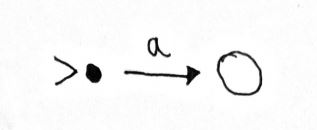
\includegraphics[scale=0.5]{a}
				\item $a \lor b$ \\ 
				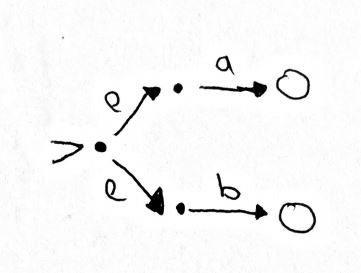
\includegraphics[scale=0.5]{aorb}
				\item $ab$ \\
				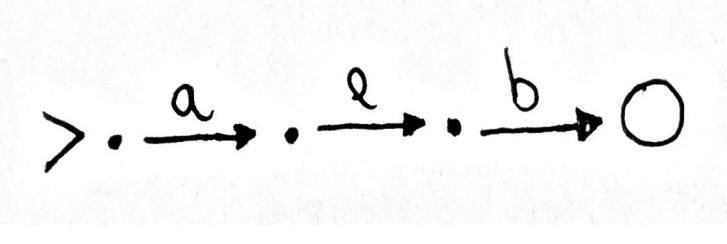
\includegraphics[scale=0.25]{ab}
				\item $a^*$ \\
				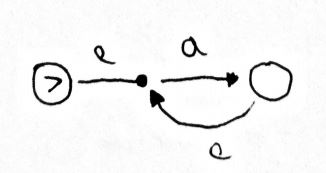
\includegraphics[scale=0.5]{astar}
			\end{itemize}
			These can be used as building blocks to construct fa for more complex regular expressions. When two of these are chained together, a new state must be added where all final states can reach this new state using $e$.\footnote{See worksheet problem 2 for example.}
		\subsection{Simplifying dfa}
		We outline a process for simplifying a dfa. By simplifying we mean producing a new dfa with a possibly smaller number of states that accepts the same language.\footnote{See worksheet problem 8 for example.}
		\begin{enumerate}
			\item Partition the states into $P_0$ composed of two partitions, one with the final states $F$ and the other with the non-final states $\overset{~}{F}$
			\item List the behavior of each state $s \in S$ under each character $a \in A$
			\item Partition $P_0$ into $P_1$ such that each state in each partition leads to the same partition when consuming $a \in A$ \footnote{That is to say, all states in a partition must go to the same other partition given a character $a \in A$.}
			\item Repeat 3. until no new partitions are formed
			\item Draw a dfa where each partition is a state, the partition including $S_0$ is the initial state, and any partition such that $P \subset F$ is a final state  
		\end{enumerate}
		\subsection{Finding Language of f.a.}
	We define a recursive procedure for finding the language accepted by an arbitrary f.a.\footnote{See worksheet problem 4 for example.} For any two states $i$ and $j$ and intermediate states up to $k$, the words that take the f.a. from state $i$ to $j$ using intermediate states up to at most $k$ is given by 
	$$R(i,j,k) = R(i,j,k-1) \cup R(i,k,k-1)R(k,k,k-1)^*R(k,j,k-1)$$
	This is applied recursively to each term until $k$ goes to 0, at which point we consider only edges. In practice it is often obvious that no paths exist prior to reaching $k=0$, at which point the term can be substituted by $\O$. It is also useful to note the following properties:
	\begin{itemize}
		\item $A\cdot \O = \O$, for any set A
		\item $\O^* = \{e\}$
		\item $A \cdot \{e\} = A$, for any set A
	\end{itemize}	 
\end{document}
